\documentclass{article}
\usepackage{graphicx}
\usepackage{amsmath}

\usepackage{listings}
\usepackage{color}

\definecolor{backcolour}{rgb}{0.95,0.95,0.92}

\lstdefinestyle{mystyle}{
    backgroundcolor=\color{backcolour}
    }

\lstset{style=mystyle}

\title{Statistical Modeling 2 \\ Exercise 2}

\begin{document}
\maketitle
\section{A simple Gaussian location model}
\subsection*{A}
The joint prior over the mean parameter \(\theta\) and precision parameter \(\omega\) is:
\begin{align*}
p(\theta, \omega) \propto \omega^{(d+1)/2-1} \exp \left\lbrace -\omega\frac{\kappa(\theta-\mu)^2}{2}\right\rbrace \exp \left\lbrace -\omega\frac{\eta}{2} \right\rbrace
\end{align*}
To get the marginal prior, we integrate out the parameter \(\omega\):
\begin{align*}
p(\theta) &\propto \int_0^{\infty} \omega^{(d+1)/2-1} \exp \left\lbrace -\omega\frac{\kappa(\theta-\mu)^2 + \eta}{2}\right\rbrace\\
&\propto \left(\frac{\kappa(\theta-\mu)^2 + \eta}{2}\right)^{-(d+1)/2} \\
&= \left(\frac{\eta}{2} + \frac{\kappa(\theta-\mu)^2}{2}\right)^{-(d+1)/2} \\
&= \left(1 + \frac{\kappa(\theta-\mu)^2}{\eta}\right)^{-(d+1)/2} \left(\frac{\eta}{2}\right)^{-(d+1)/2} \\
&\propto \left(1 + \frac{\kappa(\theta-\mu)^2}{\eta}\right)^{-(d+1)/2}\\
&=\left(1 + \frac{1}{d}\frac{d\kappa(\theta-\mu)^2}{\eta}\right)^{-(d+1)/2}\\
\end{align*}

Let \(\nu = d, m = \mu\) and \(s = \sqrt{\eta/(d\kappa)}\), we have a Student t distribution with \(\nu\) degrees of freedom and scale \(s\):
\begin{align*}
p(\theta) \propto \left(1 + \frac{1}{\nu}\frac{(\theta-m)^2}{s^2}\right)^{-(\nu+1)/2}\\
\end{align*}

\subsection*{B}
The sampling model is:
\begin{align*}
(y_i\mid \theta, \omega) \sim N(\theta, 1/\omega)
\end{align*}
where \(y_1, \dots, y_n\) are the datapoints, \(\theta\) is the mean and \(\omega\) is the precision. We have that the likelihood for all the datapoints can be written as:
\begin{align*}
p(\mathbf{y} \mid \theta, \omega) &\propto \prod_{i=1}^n \omega^{1/2} \exp \left\lbrace -\frac{1}{2}\omega (y_i - \theta)^2 \right\rbrace\\
&= \omega^{n/2} \exp \left\lbrace -\frac{1}{2}\omega \sum_{i=1}^n (y_i - \theta)^2 \right\rbrace\\ 
&= \omega^{n/2} \exp \left\lbrace -\frac{1}{2}\omega \left( \sum_{i=1}^n y_i^2 + \sum_{i=1}^n\theta^2 - 2\sum_{i=1}^n y_i\theta\right) \right\rbrace\\ 
&= \omega^{n/2} \exp \left\lbrace -\frac{1}{2}\omega \left( \sum_{i=1}^n y_i^2 + n\theta^2 - 2n\overline{y}\theta + n\overline{y}^2 - n\overline{y}^2 \right) \right\rbrace\\ 
\end{align*}
where \(\overline{y} = \left(\sum_{i=1}^n y_i\right)/n\). Let \(S_y = \sum_{i=1}^n (y_i - \overline{y})^2\), we have:
\begin{align*}
S_y &= \sum_{i=1}^n y_i^2 + n \overline{y}^2 - 2 \sum_{i=1}^n y_i \overline{y}\\
&= \sum_{i=1}^n y_i^2 - n\overline{y}^2
\end{align*}
Therefore, the likelihood is:
\begin{align*}
p(\mathbf{y} \mid \theta, \omega) &= \omega^{n/2} \exp \left\lbrace -\frac{1}{2}\omega \left[ S_y + n(\theta^2 - 2\overline{y}\theta + \overline{y}^2) \right] \right\rbrace\\ 
&= \omega^{n/2} \exp \left\lbrace -\frac{1}{2}\omega \left[ S_y +  n (\overline{y} - \theta)^2\right] \right\rbrace\\ 
\end{align*}

The posterior is proportional to the product of the likelihood and the prior:
\begin{align*}
p(\theta, \omega \mid \mathbf{y}) &\propto \omega^{(d+1)/2 - 1} \exp\left\lbrace - \omega \frac{\kappa(\theta-\mu)^2}{2} \right\rbrace \exp\left\lbrace -\omega \frac{\eta}{2}\right\rbrace\\
&\omega^{n/2} \exp \left\lbrace -\frac{1}{2}\omega \left[ S_y +  n (\overline{y} - \theta)^2\right] \right\rbrace\\ 
&= \omega^{(d+n+1)/2 - 1}\exp\left\lbrace - \omega \frac{\kappa(\theta-\mu)^2 + n(\theta - \overline{y})^2}{2} \right\rbrace \exp\left\lbrace -\omega \frac{\eta + S_y}{2}\right\rbrace\\
\end{align*}

We also have:
\begin{align*}
\kappa(\theta-\mu)^2 + n (\theta - \overline{y})^2 &= \kappa\theta^2 + \kappa\mu^2 - 2\kappa\theta\mu + n\theta^2 + n\overline{y}^2 - 2n\theta\overline{y}\\
&= (\kappa + n)\theta^2 - 2\theta(\kappa\mu + n\overline{y}) + (\kappa\mu^2 + n\overline{y}^2)\\
&=(\kappa+n)\left( \theta^2 - 2 \theta \frac{\kappa\mu + n\overline{y}}{\kappa + n} + \frac{(\kappa\mu + n\overline{y})^2}{(\kappa + n)^2} \right) - \frac{(\kappa\mu + n\overline{y})^2}{\kappa + n} + (\kappa\mu^2 + n\overline{y}^2)\\
&= (\kappa+n)\left( \theta^2 -\frac{\kappa\mu + n\overline{y}}{\kappa + n}\right)^2 - \frac{(\kappa\mu + n\overline{y})^2}{\kappa + n} + (\kappa\mu^2 + n\overline{y}^2)\\
\end{align*}


Therefore, the posterior is:
\begin{align*}
p(\theta, \omega \mid \mathbf{y}) &\propto \omega^{(d^*+1)/2 - 1} \exp\left\lbrace - \omega \frac{\kappa^*(\theta-\mu^*)^2}{2} \right\rbrace \exp\left\lbrace -\omega \frac{\eta^*}{2}\right\rbrace\\
\end{align*}
where:
\begin{align*}
&d^* = d + n\\
&\kappa^* = \kappa + n\\
&\mu^* = \frac{\kappa\mu + n\overline{y}}{\kappa + n}\\
\end{align*}
and
\begin{align*}
\eta^* &= \eta + S_y - \frac{(\kappa\mu + n\overline{y})^2}{\kappa + n} + (\kappa\mu^2 + n\overline{y}^2)\\
&= \eta + S_y + \frac{(\kappa+n)(\kappa\mu^2 + n\overline{y}^2) - \kappa^2\mu^2 - n^2\overline{y}^2 + 2\kappa n\mu \overline{y} }{\kappa + n}\\
&= \eta + S_y + \frac{\kappa n\mu^2 + \kappa n\overline{y}^2 + 2\kappa n\mu \overline{y} }{\kappa + n}\\
&= \eta + S_y + \frac{\kappa n (\mu + \overline{y})^2}{\kappa + n}
\end{align*}

\subsection*{C}
The conditional distribution is:
\begin{align*}
p(\theta \mid \mathbf{y}, \omega) &\propto \exp\left\lbrace - \omega \frac{\kappa^*(\theta-\mu^*)^2}{2} \right\rbrace
\end{align*}
We see that this is a Normal distribution with mean \(\mu^*\) and variance \(1/(\omega\kappa^*)\).

\subsection*{D}
The marginal posterior of \(\omega\) is:
\begin{align*}
p(\omega \mid \mathbf{y}) &= \int_{-\infty}^{\infty} p(\omega, \theta \mid \mathbf{y}) d\theta\\
&\propto \omega^{(d^*+1)/2 - 1}\exp\left\lbrace -\omega \frac{\eta^*}{2}\right\rbrace \int_{-\infty}^{\infty} \exp\left\lbrace - \omega \frac{\kappa^*(\theta-\mu^*)^2}{2} \right\rbrace d\theta\\
&\propto \omega^{(d^*+1)/2 - 1}\exp\left\lbrace -\omega \frac{\eta^*}{2}\right\rbrace \tag{Gaussian integral}
\end{align*}
We see that this marginal is a Gamma distribution with parameter \((d^*/2, \eta^*/2)\).
\subsection*{E}
The marginal posterior of \(\theta\) is:
\begin{align*}
p(\theta \mid \mathbf{y}) &= \int_0^{\infty} p(\theta, \omega \mid \mathbf{y}) d\omega\\
&= \int_0^{\infty} \omega^{(d^*+1)/2-1} \exp \left\lbrace -\omega\frac{\kappa^*(\theta-\mu^*)^2 + \eta^*}{2}\right\rbrace\\
\end{align*}
This is the same integral in part A. By the results in A, we can see that this marginal is a Student t distribution with parameters \(\nu = d^*, m = \mu^*\) and \(s = \sqrt{\eta^*/(\kappa^* d^*)}\).

\subsection*{F}
FALSE. As \(\kappa\) approaches \(0\), the Normal prior on \(\theta\) approaches a point distribution but the density at that point is infinite. As \(d\) and \(\eta\) approach \(0\), the Gamma prior on \(\omega\) also approach a point distribution with infinite density.

\subsection*{G}
TRUE. By the results in D and E, we see that when the prior parameters approach \(0\), the posterior parameters are not \(0\) then \(p(\theta \mid \mathbf{y})\) and \(p(\omega \mid \mathbf{y})\) are valid distribution.


\subsection*{H}
The classical frequentest confidence interval for \(\theta\) is:
\begin{align*}
\overline{y} \pm t^*\frac{\sqrt{S_y}}{\sqrt{n(n-1)}}
\end{align*}

%the sampling model approaches a Normal distribution with infinite variance. 
As the prior parameters \(\kappa, d, \eta\) approach \(0\), we have the Bayesian credible interval for \(\theta\) is:
\begin{align*}
m \pm t^*s
\end{align*}
from the results in B and E, we have
\begin{align*}
m = \mu^* = \overline{y}
\end{align*}
and
\begin{align*}
s = \sqrt{\eta^*/(\kappa d^*)} = \sqrt{\frac{S_y}{n^2}}
\end{align*}
We see that this is different from the classical confidence interval.
\section{The conjugate Gaussian linear model}
\subsection*{A}
%The conditional posterior is proportional to the conditional prior times the likelihood:
\begin{align*}
p(\beta, \mathbf{y} \mid \omega) &= p(\beta \mid \omega) p(\mathbf{y} \mid \beta, \omega)\\
&= N(\beta; m, (\omega K)^{-1}) N(\mathbf{y}; X\beta, (\omega\Lambda)^{-1})\\
&\propto \omega^{p/2} K^{p/2} \exp \left\lbrace\frac{1}{2}(\beta - m)^T\omega K (\beta - m) \right\rbrace \\
&  \omega^{n/2} \Lambda^{n/2} \exp \left\lbrace\frac{1}{2}(\mathbf{y} - X\beta)^T\omega \Lambda (\mathbf{y} - X\beta) \right\rbrace \\
&= \omega^{(n+p)/2} K^{p/2} \Lambda^{n/2} \exp \left\lbrace \frac{1}{2}\omega E  \right\rbrace \\
\end{align*}
where we have let \(E\) be the sum of two quadratic forms inside the exponent:
\begin{align*}
E &= \beta^T K \beta  - 2 \beta^T K m + m^T K m + \mathbf{y}^T \Lambda \mathbf{y} - 2 \beta^T X^T \Lambda \mathbf{y}  + \beta^T X^T \Lambda X \beta\\
%&= \beta^T (K + X^T\Lambda X) \beta - 2 \beta^T ( X^T \Lambda) \mathbf{y} - 2 \beta K m
&= \begin{pmatrix}
\beta \\ \mathbf{y}
\end{pmatrix}^T
\begin{pmatrix}
K + X^T\Lambda X & -X^T\Lambda\\
-\Lambda^T X & \Lambda
\end{pmatrix}
\begin{pmatrix}
\beta \\ \mathbf{y}
\end{pmatrix}
+ \mathrm{const}
\end{align*}
where we have ignored linear terms in \(\beta\) and \(\mathbf{y}\). We then have that (given \(\omega\)) \(\beta\) and \(\mathbf{y}\) are jointly Normal:
\begin{align*}
\begin{pmatrix}
\beta \\ \mathbf{y}
\end{pmatrix} \sim N\left( \begin{pmatrix}
m \\ Xm
\end{pmatrix}, \begin{pmatrix}
\omega K + \omega X^T\Lambda X & - \omega X^T\Lambda\\
-\omega \Lambda^T X & \omega \Lambda
\end{pmatrix}^{-1} \right)
\end{align*}

Using the conditional Normal equations, we have that \(p(\beta \mid \mathbf{y}, \omega)\) is Normal with mean:
\begin{align*}
m^* &= m + (\omega K + \omega X^T\Lambda X)^{-1}(-\omega X^T \Lambda)(Xm - \mathbf{y})\\
&= m + (K + X^T\Lambda X)^{-1}(-X^T \Lambda)(Xm - \mathbf{y})\\
\end{align*}
and variance:
\begin{align*}
(\omega K^*)^{-1} = (\omega K + \omega X^T\Lambda X)^{-1}
\end{align*}


\subsection*{B}
We have that \(p(\mathbf{y} \mid \omega)\) is Normal with mean \(X m\) and variance:
\begin{align*}
\mbox{var}(X\beta + \epsilon) &= X \mbox{var}(\beta)X^T + (\omega\Lambda)^{-1}\\
&= X (\omega K)^{-1}X^T + (\omega\Lambda)^{-1}\\
\end{align*}

We then have:
\begin{align*}
p(\omega \mid \mathbf{y}) &\propto p(\omega)  p(\mathbf{y} \mid \omega) \\
&\propto \omega^{d/2 - 1} \exp \left\lbrace - \omega\frac{\eta}{2} \right\rbrace \omega^{n/2} \exp \left\lbrace - \omega\frac{1}{2} (\mathbf{y} - Xm)^T (XK^{-1}X^T + \Lambda^{-1})^{-1} (\mathbf{y} - Xm) \right\rbrace
\end{align*}
We see that this distribution is Gamma with parameter \(d^*/2\) and \(\eta^*/2\) where:
\begin{align*}
d^* &= d + n\\
\eta^* &= \eta +  (\mathbf{y} - Xm)^T (XK^{-1}X^T + \Lambda^{-1})^{-1} (\mathbf{y} - Xm)
\end{align*}

\subsection*{C}
\begin{align*}
p(\beta \mid \mathbf{y}) &= \int_{0}^{\infty} p(\beta \mid \mathbf{y}, \omega) p(\omega \mid \mathbf{y}) d\omega\\
& \int_{0}^{\infty} \omega^{(d+n+p)/2} \exp \left\lbrace -\frac{\omega}{2}(\beta - m^*)^T K^* (\beta - m^*) \right\rbrace \exp \left\lbrace -\frac{\omega}{2} \eta^* \right\rbrace
\end{align*}
This is an integral over a Normal gamma distribution. From previous results, we see that it is a Student t distribution:
\begin{align*}
p(\beta \mid \mathbf{y}) = \left(1 + \frac{1}{\nu}\frac{(\beta-\mu)^2}{s^2}\right)^{-(\nu+1)/2}\\
\end{align*}
where 
\begin{align*}
\nu = d + n + p\\
\mu = m^*\\
s = \sqrt{\eta^*}\\
\end{align*}

\subsection*{D}
\textsc{Code: blr.r}


\begin{figure}[h!]
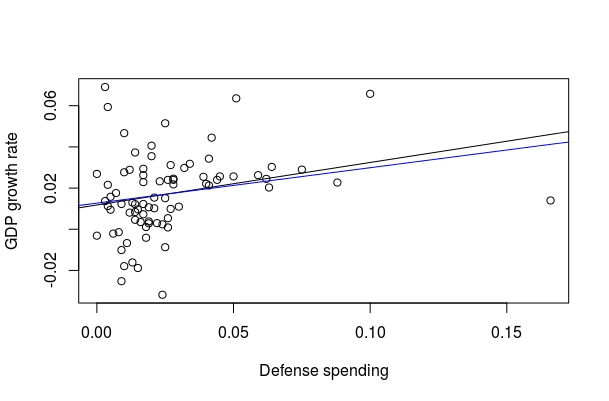
\includegraphics[width=\linewidth]{blm.jpeg}
\caption{Frequentest regression line in black and Bayesian regression line in blue.}
\label{fig:blm}
\end{figure}

\noindent
\textbf{Figure \ref{fig:blm}:} The two lines (Frequentest and Bayesian) are close on the left (Defense spending from \(0.00\) to \(0.10\)), where most of the data points are. On the right ( Defense spending from \(0.10\)), there is a greater difference, likely due to the few points available. 

\section*{A heavy-tailed error model}
\subsection*{A}
With the Gamma parameters \(\lambda\) integrated out, the marginal distribution over \(y_i\) is Student t. It has a wider tail and is more robust to outliers.

\subsection*{B}
\begin{align*}
p(\lambda_i \mid \mathbf{y}, \beta, \omega) & \propto p(\lambda_i, y_i, \beta, \omega)\\
&= p(\omega) p(\lambda_i) p(\beta \mid \omega) p(y_i |\beta , \omega, \lambda_i)\\
&\propto p(\lambda_i)  p(y_i |\beta , \omega, \lambda_i)\\
&\propto \lambda_i ^{h/2 - 1} \exp \left(- \lambda_i h/2 \right) (\omega \lambda_i)^{1/2} \exp \left[ -\frac{1}{2} \omega \lambda_i (X_i^T\beta - y_i)^2 \right]\\
&\propto \mathrm{Gamma}\left(\frac{h+1}{2}, \frac{1}{2}[h + \omega (X_i^T\beta - y_i)^2]\right)
\end{align*}
\subsection*{C}
\textsc{Code: heavy\_tail.r}

\begin{figure}[h!]
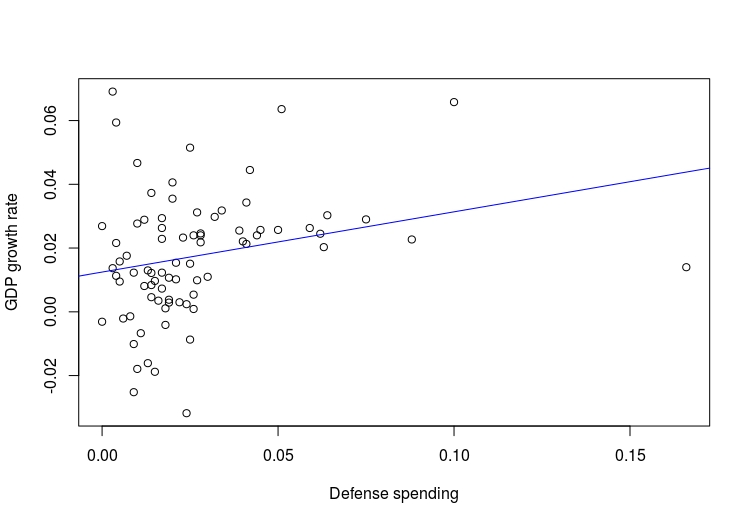
\includegraphics[width=\linewidth]{heavy_tail.jpeg}
\caption{Regression line fitted by Gibbs sampling.}
\label{fig:heavy}
\end{figure}

\noindent
\textbf{Figure \ref{fig:heavy}:} Compare to the lines in Figure \ref{fig:blm}, this line seems to be less affected by the outliers.

\end{document}